\section{模型建立与求解}
\subsection{特征选择与分布检验}
\subsubsection{特征选择}
原始的数据集中特征个数为95,不仅特征数量较多,同时存在方差较小、相关性较强的
特征,不利于直接使用机器学习算法进行类别预测。从协方差矩阵热度图中观察到,特征与
是否破产(标签)之间的线性相关性普遍较弱,直接利用协方差数值进行选择的方式难以
奏效。基于这两点观察,分两阶段进行特征选择:
\begin{enumerate}
    \item 去除方差较小(方差$<0.15$)的特征,对于线性相关性较强的特征
    (协方差矩阵中数值$\geq 0.8$),保留其中任意一个;
    \item 利用互信息对特征进行评分,选择排名前30\%的特征。互信息可以捕捉单个特征与目标之间的非线性关系,但是没有考虑特征之间的高阶
    相关性。由于没有对数据的分布做先验假设,这使得其相对\textit{F}检验等假设检验方法
    可以适用于更多的场景。由于第一阶段筛选后的特征数量仍然较多,对于每个特征
    做正态分布的检验较为繁琐,所以选择使用互信息作为评分标准。
\end{enumerate}
互信息利用\textit{KL}散度衡量概率分布$p(x_i, y)$和$p(x_i)p(y)$的相近程度:
\begin{equation*}
MutualInformation(x_i,y) = KL(p(x_i, y) \ \| \ p(x_i)p(y))
\end{equation*}
其中$x_i$是第$i$个特征,$y$是标签。
对于连续型分布$p(x),q(x)$,\textit{KL}散度表示为:
\begin{equation}
    KL(p\ \|\ q)=\int_{-\infty}^{\infty} p(x)\log\frac{p(x)}{q(x)} \,dx 
    \label{eq:KL-divergence}
\end{equation}
式\ref{eq:KL-divergence}推广到本题的情况即是:
\begin{equation}
S(x_i)\coloneqq 
\sum\limits_{y\in\mathcal{Y}} 
\int_{-\infty}^{\infty} p(x_i,y)\log\frac{p(x_i)p(y)}{p(x_i,y)} \,dx 
    \label{eq:score-mutual-information}
\end{equation}
其中:
\begin{itemize}
    \item $S(x_i)$是特征$x_i$的互信息得分,得分高的变量会被最终选取
    \item $\mathcal{Y}$是标签的取值集合,在本题的二分类问题中,$\mathcal{Y}=\{0,1\}$
\end{itemize}
根据式\ref{eq:score-mutual-information},如果$x_i$和$y$独立,
$KL(p(x_i,y)\ \|\ p(x_i)p(y))=0$,从而变量$x_i$的得分是零,也即$x_i$不会被
选择。根据互信息得到的变量得分排序展示在图\ref{fig:score-mutual-info}中。
\begin{figure}[ht]
    \centering
    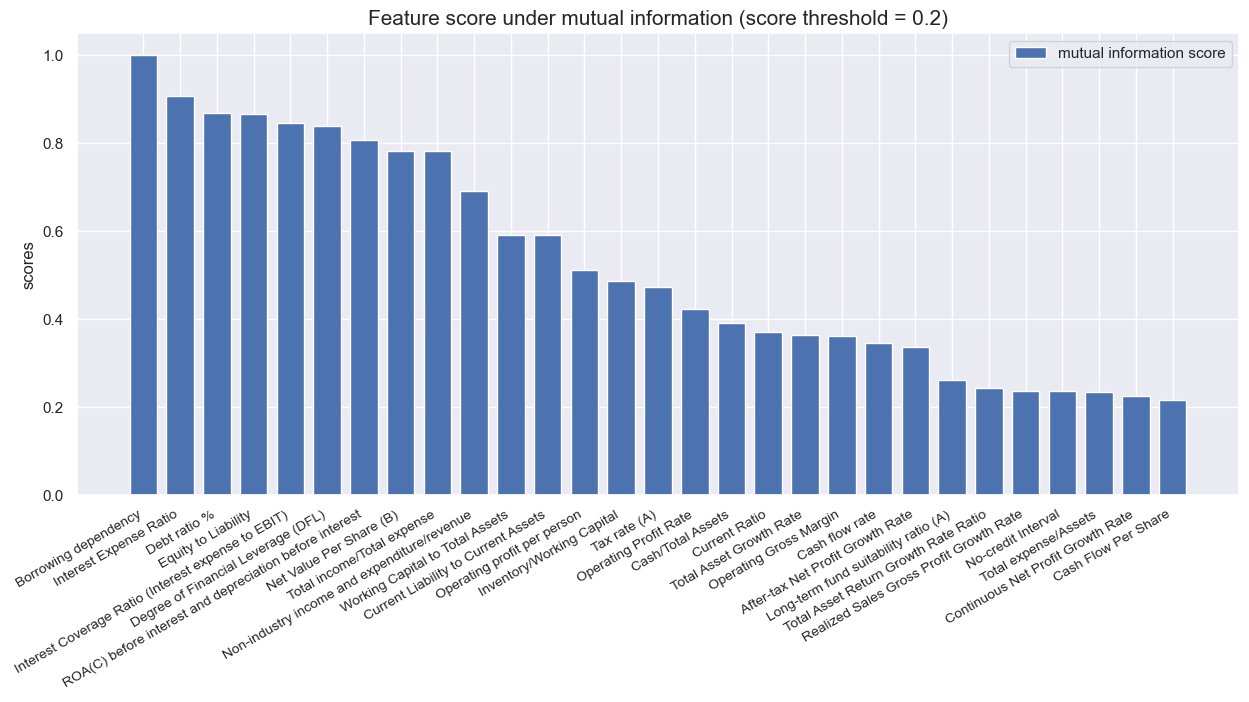
\includegraphics[width=.8\textwidth]{images/score_mutual_info.png}
    \caption{各变量互信息得分,得分阈值设定为0.2(小于阈值的变量不予以展示)}
    \label{fig:score-mutual-info}
\end{figure}
从图\ref{eq:score-mutual-information}中看出,与公司运营情况相关性最强的
五个因素为(按得分先后顺序):
\begin{enumerate}
    \item \textbf{Borrowing Dependency}: 借贷依赖,衡量公司对于贷款的依赖
    程度
    \item \textbf{Interest Expense Ratio}: 利息费用比率,衡量公司的
    利润中多大比例用于偿还贷款利息
    \item \textbf{Debt Ratio}: 资产负债率,衡量公司总资产中贷款的比例
    \item \textbf{Equity to Liability}: 权益对负债比率,衡量股东的资产对于
    公司债务、贷款的比例
    \item \textbf{ROA(C) Before Interest and Depreciation}: 资产变现率,
    衡量公司资产用于产生利润的比例
\end{enumerate}
根据经济学知识,以上五个变量在衡量公司资本结构、资产回报、盈利能力上发挥着
重要的作用。但是基于统计理论的特征选择不一定总能够在经济理论中获得解释,
这反映出特征选择容易受到不稳定数值的影响。

\subsubsection{特征分布检验}
对于互信息选择的18个特征进行高斯分布检验。
检验前将数据标准化,再使用Q-Q图进行正态性检验,
将互信息得分排名前二的两个特征的检验结果展示在图\ref{fig:qqplot-gaussian}中。
\begin{figure}[ht]
    \centering
    \begin{minipage}[c]{0.45\textwidth}
        \centering
        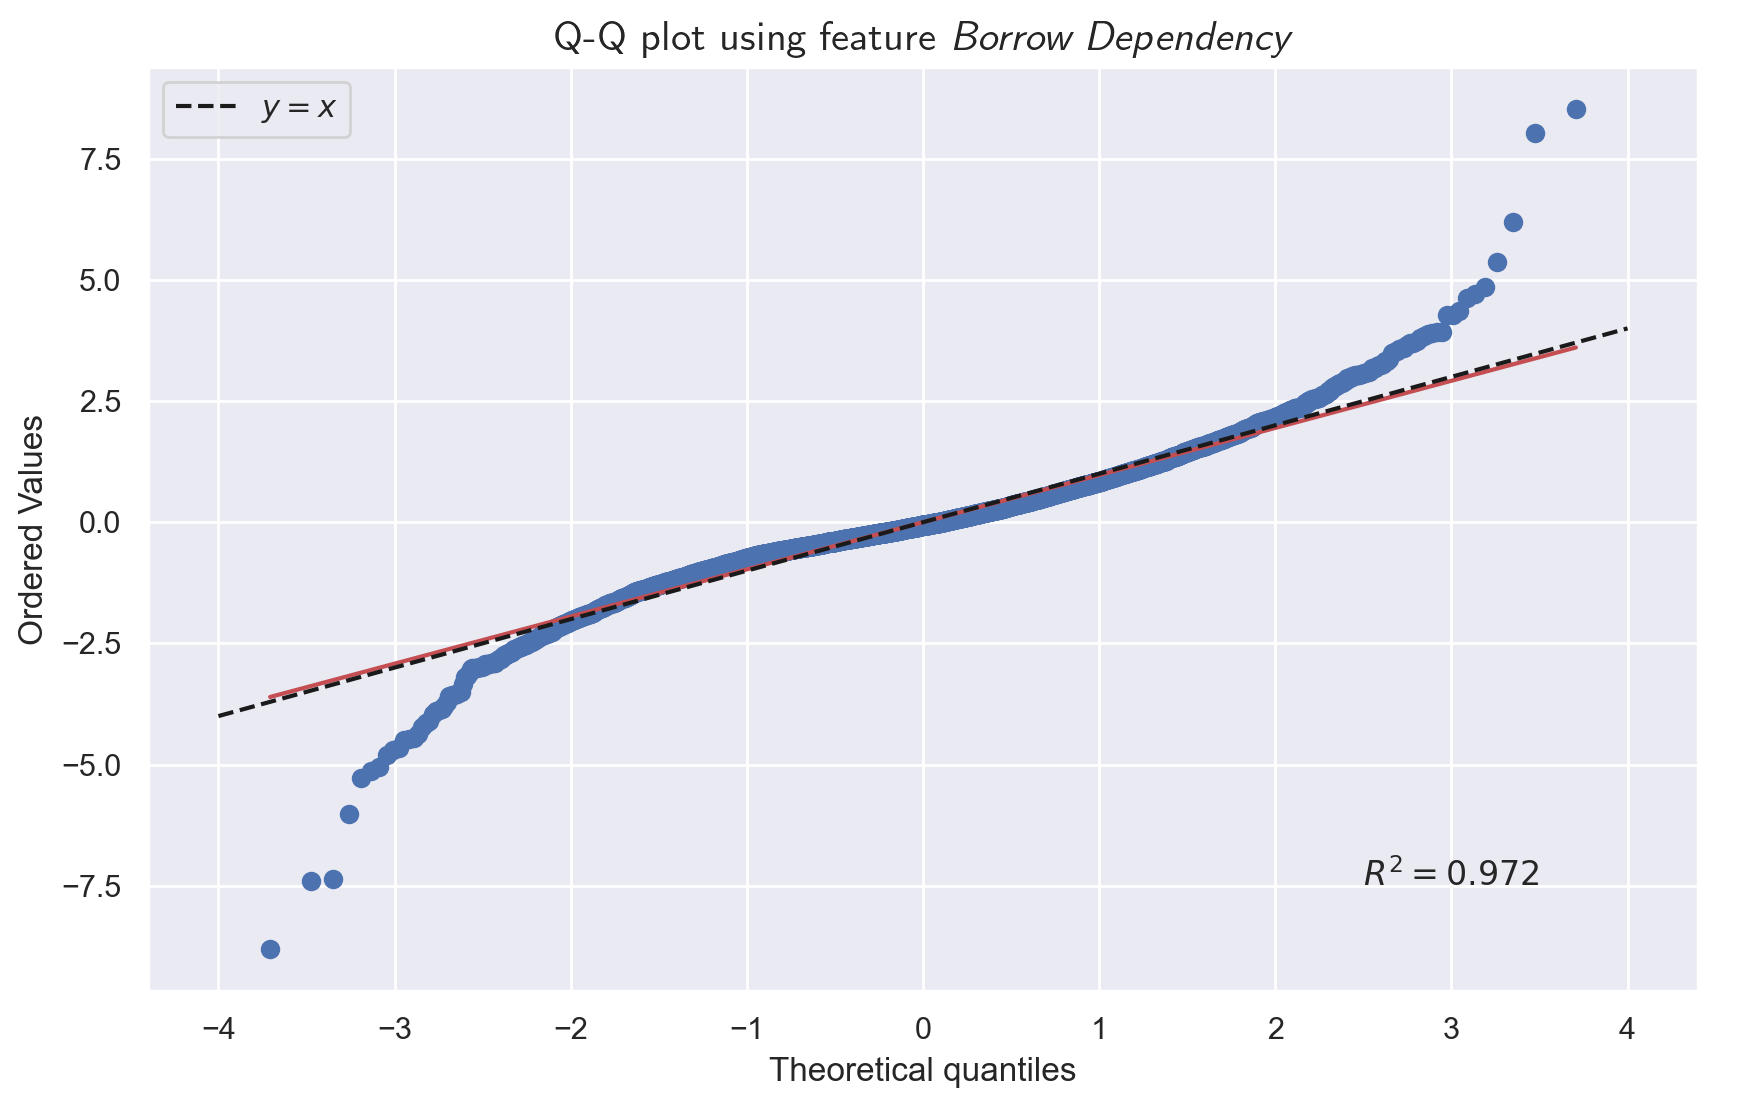
\includegraphics[width=0.9\textwidth]{images/qqplot_borrow_dependency.png}
        \subcaption{借贷依赖正态性检验}
        \label{fig:borrow-dependency-qq}
    \end{minipage}
    \begin{minipage}[c]{0.45\textwidth}
        \centering
        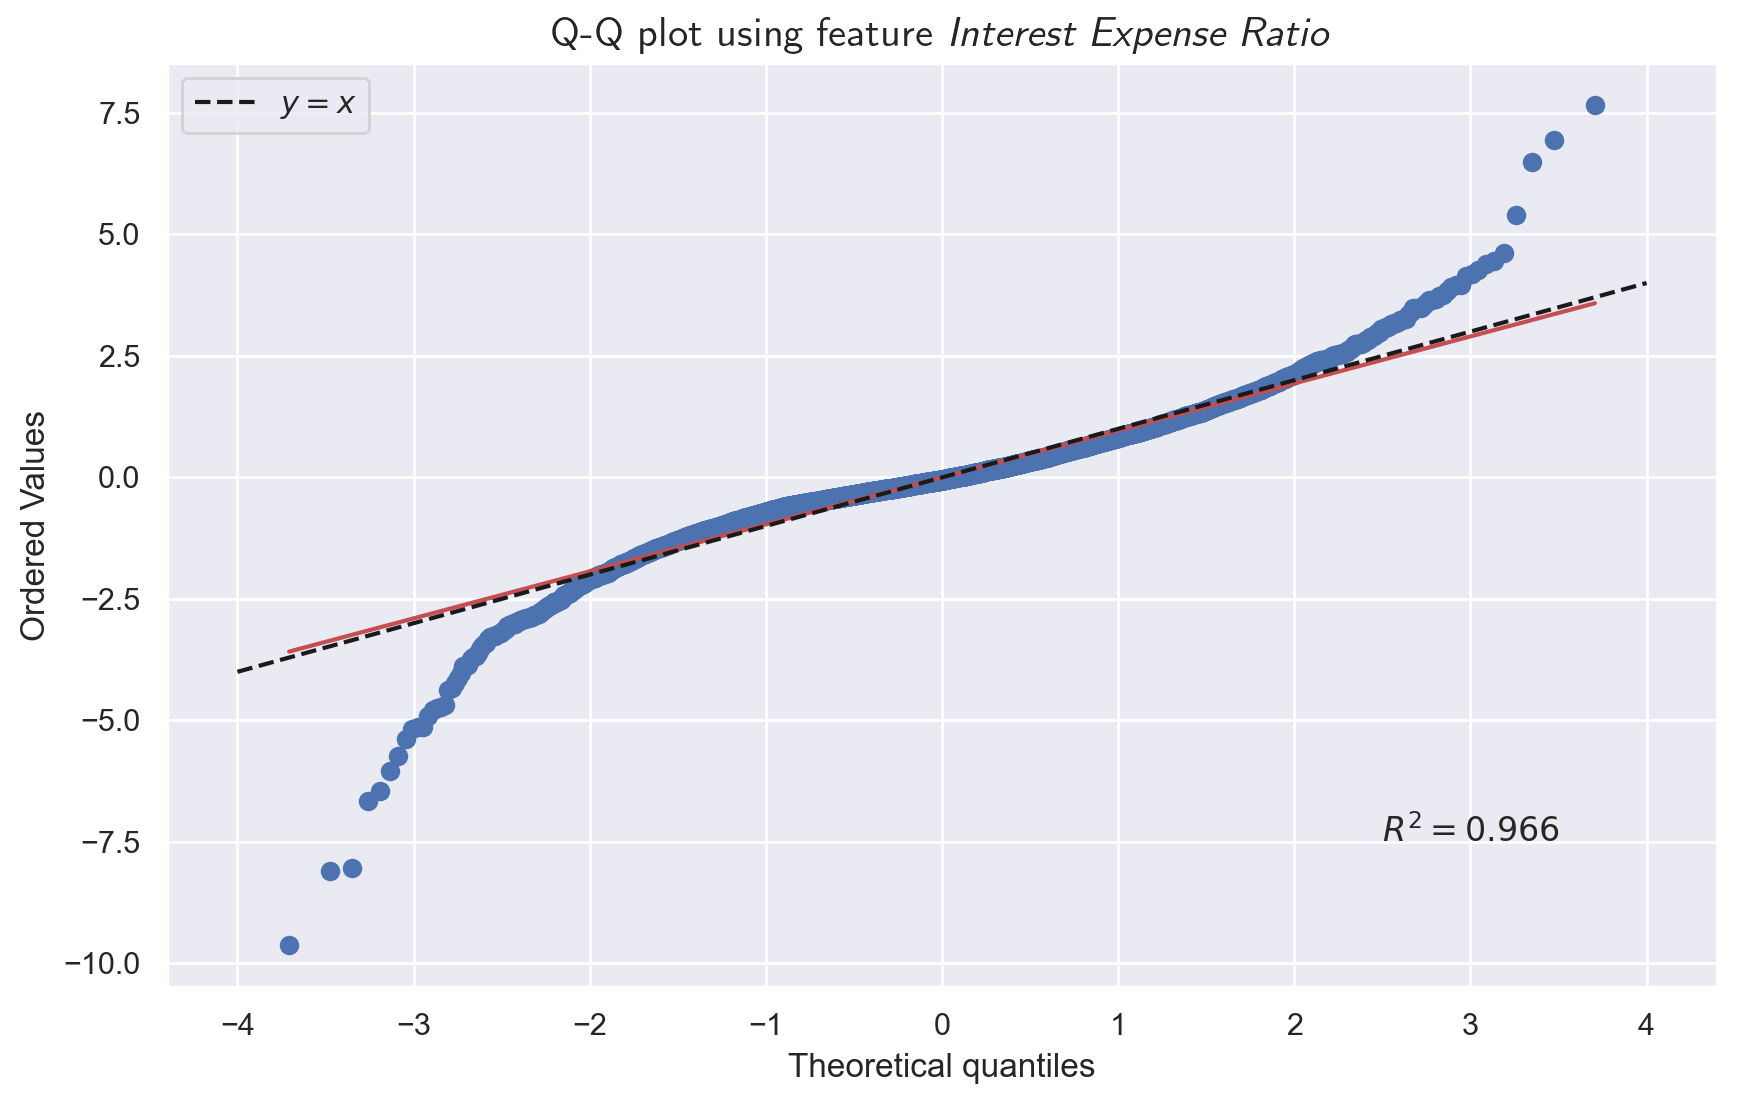
\includegraphics[width=0.9\textwidth]{images/qqplot_interest_expense_ratio.png}
        \subcaption{利息费用比率正态性检验}
        \label{fig:interest-expense-qq}
    \end{minipage}
    \caption{特征正态性检验结果(Q-Q图)}
    \label{fig:qqplot-gaussian}
\end{figure}
从图中看出,排序后的数据点与理论分位数可以较好地使用$y=x$进行拟合,说明
数据通过正态性检验。